\section{Безопасность}
\subsection{Контроль доступа и аутентификация}

Конечное устройство (КУ) не может получить доступ к сети без предварительной идентификации (сравнением с белым или черным списком) и аутентификации. Идентификация и аутентификация строятся на двух параметрах, которые однозначно определяют КУ:

\begin{itemize}
 \item адрес EUI-48 MAC, описанный в IEEE 802-2001. Данный адрес легко перевести в адрес EUI-64 (описан в IEEE 802.15.4 и связанных с ним документах);
 \item 128-битный общий ключ (предварительный ключ или PSK) используемый как удостоверение в процессе аутентификации. Данный ключ находитяс на КУ и сервере. Аутентификация базируется на проверке PSK сервером и подтверждением для КУ что сервер знает PSK, тоесть происходит взаимная аутентификация. Сам PSK держется в секрете.
\end{itemize}

Процес идентификации и аутентификации запускается при перезапуске КУ и, также, может быть запущен в любой момент сгласно политике безопасности. Все данные для идентификации и аутентификации передаются при помощи самонастраевоемого протокола 6LoWPAN(LBP) (пункт 9.4.4) который внедряет собственный расширяемый протокол аутентификации(EAP) (пункт 9.4.4.2.1.2).

Как показано на рисунке \ref{img:10-1}, LBP и EAP были разработаны так, что бы передаваться по промежуточным узлам. Так, в начале фазы самонастройки, если КУ ещё не получило собственный 16-битный адресс на расстоянии 1 прыжка от PAN координатора(LBS), они всё равно могут общаться напрямую. В иных случаях они должны использовать промежуточный узел(LBA), расположенном на растоянии одного прыжка от LBD.

Кроме того, должны быть продуманы две другие архитектуры механизма аутентификации:
\begin{itemize}
 \item Функция сервера аутентификации непосредственно поддерживается LBS и тогда все материалы для аутентификации(списки доступа, полномочия и т.д.) должны быть загружены в LBS;
 \item Функция сервера аутентификации поддеривается удаленным(централизованно) AAA сервером, в данном случае LBS только отвечает за пересылку EAP сообщений на AAA сервер по стандартному AAA протоколу (то есть RADIUS [IETF RFC 2865]).
\end{itemize}
\begin{figure}[h]
\center{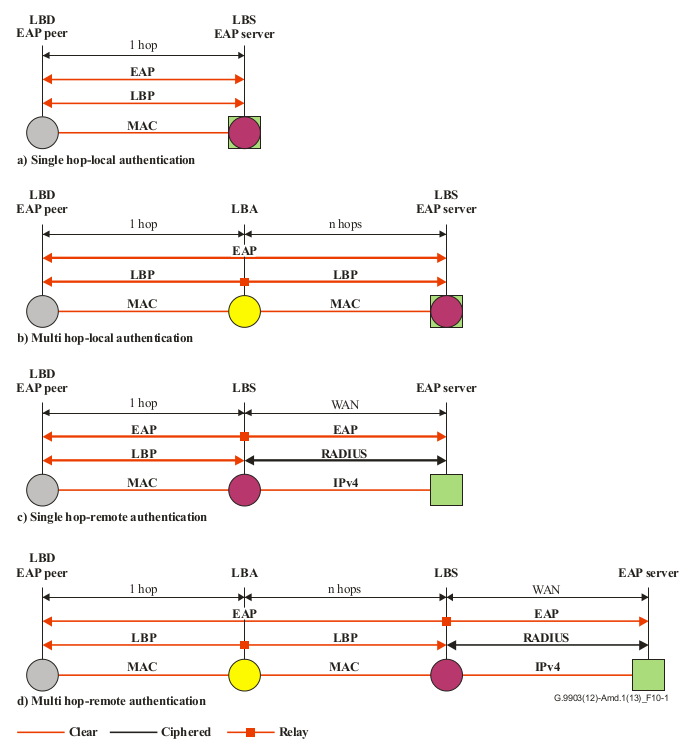
\includegraphics[width=0.9\linewidth]{./pictures/10-1}}
\caption{возможности ретрансляции LBP и EAP}
\label{img:10-1}
\end{figure}

Процес аутентификации целиком зависит от метода EAP. EAP протокол очень гибкий и поддерживает различные методы EAP (EAP-MD5, EAP-AKA, EAP-TLS, и т.д.). Каждый метод характериуется своими учетными данными (общий секрет, сертификат, SIM-карта, и т.д.), его сертификатом и алгоритмом шифрования.

Для данной редакции принят метод EAS-PSK (пункт 10.5), основными целями которого является:
\begin{itemize}
 \item Простота: он основан на общем 128-битном секрете и алгоритме шифрования AES-128;
 \item Безопасность: очень консервативен и основывается на проверенных и надежный криптосистемах;
 \item Расширяем: в этой редакции, имеет возможность расширения на механизм группового распределения ключей (пункт 10.5.2).
\end{itemize}

\subsection{Целостность и конфиденциальность}

Как показанно на рисунке \ref{img:10-2}, конфиденциальность и целостность обеспечиваются на различных уровнях:
\begin{itemize}
 \item На MAC-уровне: как определенов в [IEEE 802.15.4], CCM* алгоритм шифрования, применяемый к каждому кадру, передаваемому между узлами сети. Это универсельный, низкоуровневый сервис обеспечения конфиденциальности и целостности. MAC кадрый расшифровываются и зашифровываются при передачи от узла к узлу. Исключением являютмя только некоторые служебные кадры, передаваемые на этапе самонастройки. Достаточным условием поддержки данной функции является наличие на каждом узде группового мастер ключа(GMK). GMK доставляется на каждый узел индивидуально при помощи защищенных каналов EAP-PSK;
 \item На EAP-PSK уровне: как определено в [IETF RFC 4764], EAP-PSK обеспечивает конфиденциальность и целостность (и защиту от повторов), также известные как защищенный канал (PCHANNEL) для сообщений, которыми обмениваются в процессе EAP EAP-сервер и его клиенты.
\end{itemize}

\begin{figure}[h]
\center{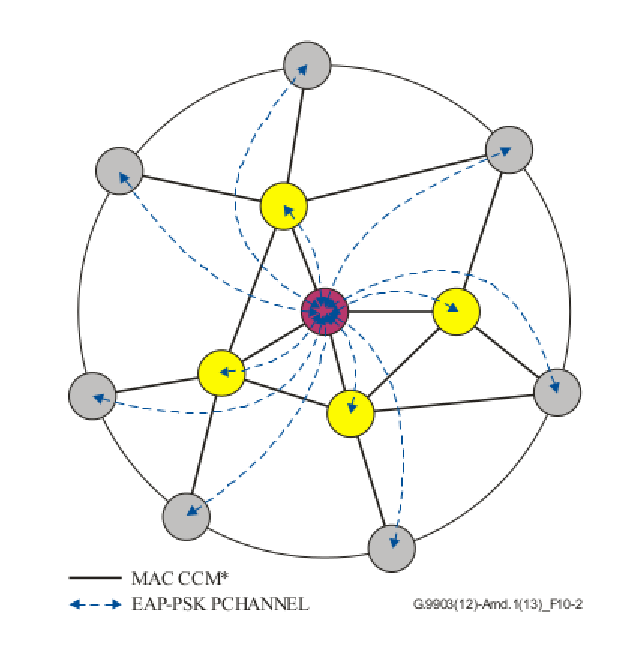
\includegraphics[width=0.9\linewidth]{./pictures/10-2}}
\caption{Конфиденциальность и безопасность}
\label{img:10-2}
\end{figure}

\subsection{Защита от повторов и рофилактика DoS атак}

Предотвратить DoS атаку всегда сложно, особенно если она направлена на физический уровень. Но на данном уровне воздействие такой атаки ограничено небольшой областью.

CCM* шифрование распространяется на весь MAC уровень. Это предотвращает доступ в сеть неавторизованных и оказывающих влияние на маршрутизацию и другие низкоуровневые процессы устройств. Единственным исключением является доверенный процесс автонастройки. Кроме того, на подуровне MAC задается механизм контроля за повторной отправкой сообщений.

\subsection{Аутентификация и протокол распределения ключей - выборка из IETF RFC 3748}

Аутентификация и распространение ключей поддерживается протктолом расширенной аутентификации (EAP) как указанов в [IETF RFC 3748] совместно с парамерами, представленной в таблице 1.%\ref{tab:10-1}.

\begin{longtable}{|l|p{0.7\linewidth}|l|}
 %\begin{center}
  \caption{Выборка из IETF RFC 3748} \\ %\label{tab:10-1}\\
  %\endfirsthead
  %\begin{tabular}{|l|p{0.7\linewidth}|l|}
   \hline 
   Пункт & Название и замечания & Определение \\
   \hline
   %\endhead
   1 & Введение  & N \\
   \hline
   2 & Расширяемый протокол аутентификации (EAP) & S \\ & - первоначальный идентифицирующий запрос позволяющий начать процедуру аутентификации.& \\
   \hline 
   2.1 & Поддержка последовательностей & N \\
   \hline
   2.2 & Модель мультиплексирования EAP & S \\ & - определена только одна EAP модель (9.4.4) &  \\
   \hline
   2.3 & Отношение прямого доступа & S \\ & - над LBP поле немного отлечается от обычного EAP поля, описанного в [IETF RFC 3748]. Присутствует двустороннее преобразования данного поля которое происходит при передачи EAP сообщения по сторонним протоколам (например RADIUS) и в случае защиты области заголовка EAP &  \\
   \hline
   2.4 & Операции ``точка - точка'' & N \\
   \hline
   3 & Взаимодействие на нижнем уровне & N \\
   \hline 
   3.1 & Требования нижнего уровня & S \\ & LBP и вложенные протоколы обеспечивают: & \\
    & - надежность передачи; & \\
    & - обнаружение ошибок (CRC); & \\
    & - нет обеспечения безопасности при автонастройке; & \\
    & - размер MTU превышает 1020 октетов (с фрагментацией); & \\
    & - отсутствие дублирования; & \\ 
    & - гарантия доставки. & \\
   \hline
   3.2 & Использование EAP c PPP & N/R \\
   \hline
   3.3 & Использование EAP с IEEE 802 & N/R \\
   \hline
   3.4 & Сигналы нижнего уровня & N \\
   \hline
   4 & Формат покета EAP & S \\
   & -  & \\
   \hline
   4.1 & & S \\
   \hline
   4.2 & & S \\
   \hline
   4.3 & & N \\
   \hline
   5 & & S \\
   \hline
   5.1 & & N/R \\
   \hline
   5.2 & & N/R \\
   \hline
   5.3 & & N \\
   \hline
   5.4 & & N/R \\
   \hline
   5.5 & & N/R \\
   \hline
   5.6 & & N/R \\
   \hline
   5.7 & & N/R \\
   \hline 
   5.8 & & N/R \\
   \hline
   6 & & N \\
   \hline
   7 & & N \\
   \hline
   8 & & I \\
   \hline
   9 & & N \\
   \hline
   Приложение А & & I \\
   \hline    
  %\end{tabular}
 %\end{center}
\end{longtable}
